% !TeX program = lualatex
\documentclass[a5paper,11pt,openany]{article}
\usepackage{orcidlink}

\usepackage{blindtext}
%\usepackage[style]{abstract}

\usepackage[top=2cm,bottom=2cm,bindingoffset=0cm]{geometry}

\usepackage[svgnames]{xcolor} % Required to specify font color

%\documentclass[a4paper,12pt,openany]{scrbook}

%\usepackage{glossaries}
%\usepackage[xindy]{glossaries}
%\makeglossaries

%\usepackage{odsfile,lmodern}

%\usepackage{luacode}


\usepackage{multicol}

%\usepackage{churchslavonic}
%\usepackage{polyglossia}
%\setotherlanguages{russian,churchslavonic}

\usepackage{mathtext}
\usepackage{makeidx}
%\usepackage{imakeidx}
\usepackage{longtable}
\usepackage[tc]{titlepic}

\usepackage{fontspec}

\usepackage[protrusion=true,expansion,
tracking=true,letterspace=50]{microtype}


%\usepackage{academicons}
%\usepackage{xcolor}


%\SetTracking[ spacing = {25*,166, } ]{ encoding = *, shape = sc }{ 25 }


%\usepackage{soulutf8}
%\usepackage{letterspace}

%\usepackage[toc]{appendix}
\usepackage[toc,titletoc]{appendix}
\renewcommand\appendixtocname{Приложения}
\renewcommand\appendixpagename{Приложения}

%\usepackage{xunicode}
\usepackage{xltxtra}

\usepackage[normalem]{ulem}
\usepackage{adjustbox}

\usepackage{polyglossia}
\setmainlanguage{russian}
\setdefaultlanguage{russian}
\setotherlanguage{ukrainian}
\setotherlanguage{english}
\setotherlanguage{greek}
\setotherlanguage{latin}
\setotherlanguage{polish}


\setmainfont[BoldFont={DejaVuSerif-Bold.ttf},
ItalicFont={DejaVuSerif-Italic.ttf},
 BoldItalicFont={DejaVuSerif-BoldItalic.ttf}]{DejaVuSerif.ttf}

\setromanfont[BoldFont={DejaVuSerif-Bold.ttf},
ItalicFont={DejaVuSerif-Italic.ttf},
 BoldItalicFont={DejaVuSerif-BoldItalic.ttf}]{DejaVuSerif.ttf}

\setsansfont[BoldFont={DejaVuSans-Bold.ttf},
ItalicFont={DejaVuSans-Oblique.ttf},
 BoldItalicFont={DejaVuSans-Oblique.ttf}]
{DejaVuSans.ttf}

\setmonofont[BoldFont={DejaVuSansMono-Bold.ttf},
ItalicFont={DejaVuSansMono-Oblique.ttf},
 BoldItalicFont={DejaVuSansMono-BoldOblique.ttf}]
{DejaVuSansMono.ttf}



\usepackage{enumitem}
\usepackage{indentfirst} 

\usepackage{verse}

\usepackage{graphicx}

%\usepackage[pdfpagelabels,unicode,plainpages=false]{hyperref}

\hypersetup{pdftitle=Како Владимир идолы низвергал. Петр Семилетов.}

\usepackage{bookmark} 
\usepackage{relsize}

\usepackage{tocloft,calc}
\usepackage[nottoc,numbib]{tocbibind}


\frenchspacing
\righthyphenmin=2


\makeatletter
\@addtoreset{chapter}{part}
\makeatother  


%\titlepic{\includegraphics[width=0.50\textwidth]{cover/04.jpg}}

\title{КАК ВЛАДИМИР\\  ИДОЛОВ НИЗВЕРГАЛ\\
\textsmaller[2]{редакция 1.0}}
\author{Петр Семилетов\\ORCID:0009-0002-3901-7785 \orcidlink{0009-0002-3901-7785}}
\date{24/11/2024}



\newcommand*{\plogo}{\fbox{$\mathcal{PL}$}} % Generic publisher logo

% –  –  –  –  –  –  –  –  –  –  –  –  –  –  –  –  –  –  –  –  –  –  –  –  –  –  –  –  –  –  –  –  –  –  –  –  –  –  –  –  –  –  –  – 
%	TITLE PAGE
% –  –  –  –  –  –  –  –  –  –  –  –  –  –  –  –  –  –  –  –  –  –  –  –  –  –  –  –  –  –  –  –  –  –  –  –  –  –  –  –  –  –  –  – 

\newcommand*{\titleAT}{\begingroup % Create the command for including the title page in the document
\newlength{\drop} % Command for generating a specific amount of whitespace
\drop=0.1\textheight % Define the command as 10% of the total text height

\rule{\textwidth}{1pt}\par % Thick horizontal line
\vspace{2pt}\vspace{-\baselineskip} % Whitespace between lines
\rule{\textwidth}{0.4pt}\par % Thin horizontal line

\vspace{\drop} % Whitespace between the top lines and title
\centering
\textcolor{Red}{
{\Huge КАК ВЛАДИМИР\\
ИДОЛОВ НИЗВЕРГАЛ}\\[0.5\baselineskip] % Title line 1
%{\Large}\mbox{}\\[0.75\baselineskip] % Title line 2
%{\Huge четвертая редакция}} % Title line 3
}

\vspace{0.25\drop} 
\rule{0.3\textwidth}{0.4pt}\par 

\mbox{ }\\
редакция 1.0\\

%\includegraphics[width=0.40\textwidth]{cover/04.jpg}

\vspace{\drop} 

{\Large \textsc{Петр Семилетов\\ORCID: 0009-0002-3901-7785}}\par 


\vfill
%{\large \textcolor{Red}{\plogo}}\\[0.5\baselineskip] % Publisher logo
{\large \textsc{2024}}\par % Publisher

\vspace*{\drop} 

\rule{\textwidth}{0.4pt}\par
\vspace{2pt}\vspace{-\baselineskip} 

\rule{\textwidth}{1pt}\par 

\endgroup}


\begin{document}


\maketitle

\pagestyle{empty}


\newpage

\pagestyle{plain}

%\hrule

%\tableofcontents

%\input{pre/pre.tex}
%\input{plan-right/plan-right.tex}
%\input{plan-right/plan-right-text.tex}

\begin{abstract}
Знаменитое крещение Руси в Киеве князем Владимиром Красно Солнышко – курс на новую веру или... есть в этом какой-то подвох? Зачем Владимиру понадобилось публичное низвержение идолов в присутствии приглашенных из Корсуни христианских священников, и почему низвержение не вызвало возмущения народа против князя? Судя по всему, князь провел при этом языческий обряд.
\end{abstract}


\section{Како Владимир\\ идолов низвергал}

Я много упрощу здесь изложение, не касаясь зарубежных источников о Владимире, в частности исландских саг, где события, относящиеся к жизни князя и крещения как самого Владимира, так и Руси, описаны иначе, нежели в славянских источниках.

Иными словами, в летописях есть то, чего нет в сагах, а в сагах то, чего нет в летописях и житиях. И если наложить сведения из саг на летописи, то получится, что крещение произошло дважды, по восточному и западному обрядам, в разное время, при разных обстоятельствах. 

%Кроме этого двойного крещения, при сопоставлении Повести временных лет с сагами или например малоизвестной Летописью Панцерного и Аверки, из пучин истории всплывет большая загадка, касающаяся княгини Ольги – загадка куда б\'ольшая, нежели двойное крещение, но – сейчас речь не об этом.    

Я хочу рассмотреть крещение Руси именно таким, как оно описано в Повести временных лет и некоторых других давних славянских источниках, например в «Киевском Синопсисе»\cite{sinopsis} под редакцией Иннокентия Гизеля и «Кройнике»\cite{sofonovich01} Софоновича. Источники, на которых построена общепринятая история или которые близки к ней.

Если оценивать предшествующие крещению Руси события, то оно выглядит как геополитическая многоходовка. Напомню, что происходило, согласно официальной хронологии и основным спискам летописей.

В 985 году Владимир идет войной на Болгар. На каких именно – толком непонятно, ибо были известны Болгары на Волге, отсюда кстати и название их, поменяйте Б на В. А переселившиеся с Волги на Дунай Болгары тоже были Болгары, и там сейчас страна Болгария. 

Исследователи, как обычно, сделали самый нелогичный вывод и сейчас принято считать, что Владимир ходил на волжских Болгар. Но в летописи есть уточнение, как именно шел Владимир\footnote{Здесь и далее цитирую Повесть временных лет по Ипатьевскому списку\cite{ipat}, для удобства чтения и вёрстки преобразуя буквы старославянского алфавита в современные.}:

\begin{quotation}
\noindent Иде Володимир на Болгары с
Добрынею оуем своим в лодьях а Торкы берегом приведе на конех
\end{quotation}

Итак, Владимир выступил из Киева с уем своим (дядей своим Добрыней) в лодьях, а союзники Торки шли по берегу на конях.

Если вы посмотрите на карту, то увидите, что так можно добраться по Днепру к Черному морю, а там и Болгария. Но приплыть на лодьях в Булгарию Волжскую затруднительно! Мягко говоря.

   Войско Владимира побеждает Болгар, но Добрыня советует ему не делать их данниками, ибо, дескать, крепки Болгары, богато живут:

\begin{quotation}
\noindent суть вси в сапозех, сим дани нам не платити, поидев искать лапотник.
\end{quotation} 

   То бишь, пойдем лучше выбивать дань с кого победнее, с лапотников. Владимир заключает с Болгарами мир и возвращается в Киев.

Спустя год, в 986, согласно летописи, Болгаре прибывают в Киев и предлагают Владимиру принять их веру, а они, как пишет летопись, Бохмичи – то бишь магометане, мусульмане. Рассказывают об особенностях своей веры, но Владимир отказывается, ибо ему не нравятся два пункта. Первый это обрезание, а второй – воздержание от спиртных напитков. «Руси веселье питье не можем без того быти» – отвечает Владимир прибауткой.

   Вся летописная глава за 986 год посвящена тому, как представители разных церквей и религий ходят к Владимиру с предложениями принять их веру. Приходят «Немцы от Рима». Приходят Иудеи. Наконец от Греков – то есть из Византии, греческой ветви опять же Римской империи – от Греков прибывает некий философ, сообщает о других религиях самые неприятные сведения, и утверждает истинность восточной христианской церкви, а заодно пересказывает Библию. 

Эта глава кажется искусственно вставленной в повествование летописи, хотя возможно, в самом деле имело место посольство к Владимиру различных религиозных структур с целью обезопасить державы, где господствовали эти структуры, от набегов крепнущей Киевской Руси.

Однако напомню, что всего 6 лет назад, когда Владимир только начал княжить в Киеве, он установил идолы целого пантеона языческих богов:

\begin{quotation}
\noindent постави кумиры на холму вне двора теремнаго . Перуна деревяна а голова его серебряна а оус золот и Хорса . и Дажьбога . и Стрибога . и Семарьгла. и Мокошь . и жряху им . наричуще богы и привожаху сыны своя и жряху бесом и оскверняху землю требами своими
\end{quotation}

   Не просто поставил кумиров, но, приводил туда сыновей своих и приносил в жертву бесам. Речь идет именно об этом, ибо далее летописец говорит, «но преблагыи Бог не хотяи смерти грешником», с чего бы Нестору об этом писать, если не подразумевалось принесение в жертву сыновей, которых учитывая количество наложниц у Владимира было немеряно.

   В 980 Владимир устанавливает идолов, а в 986-м ему предлагают примкнуть к одной из авраамических религий. 

   Спустя год, в 987, Владимир посылает своих бояр разузнать, каковы же предлагаемые веры. Бояре отправляются к Болгарам, затем к Немцам, а после ко Грекам, и бояре по возвращении склоняются к мысли, что у Греков лучше всего, да и, дескать, княгиня Ольга вон была мудрее всех, а приняла христианство \textbf{греческого} обряда. Тогда Владимир спрашивает у бояр:

 – То кде крещение приимем?

 – Кде ти любо, – ответили бояре.

   Проходит год, и вот в 988 Владимир идет с воинством на греческий град Корсунь. Корсунь ныне те развалины Херсонеса, что лежат возле Севастополя. А Корсунь относилась к восточной Римской Империи, называемой в летописи Греки, а сейчас Византией. Корсунь была одним из очагов христианства и торговли.

   И вот Владимир безуспешно берет город в осаду. Стоит под стенами. Однако среди Корсунян оказался предатель – муж именем Анастас. Он послал в стан врагов, к Владимиру, стрелу с запиской:

\begin{quotation}
\noindent кладези яже суть за тобой от востока ис того вода идет по трубе копавше преимете воду
\end{quotation}

  То есть от колодца к востоку идет вода по трубе. Раскопав, перекройте воду.

   Владимир, узнав про это,

\begin{quotation}
\noindent взрев на небо и рече: аще ся сбудеть, се имам креститися
\end{quotation}

То есть воззрился на небо и сказал – если получится, то крестимся!

   Далее Владимир начнёт шантажировать императоров Василия и Константина, добиваясь крещения. В свете этого и выглядит странным летописный раздел о выборе Владимиром восточного обряда христианства среди прочих вер. Ведь если предлагали и так, зачем вынуждать силой?

   Как бы ни было, Владимир приказывает раскопать и перекрыть трубу. В Корсуни начинается большая жажда и город сдается.

   Владимир с дружиной входит в Корсунь и посылает в Царьград (Константинополь, ныне Стамбул) сообщение. Мол, вот я взял Корсунь, хотите то же самое будет с вашей столицей, Царьградом? Если нет, вот мои условия. Я слышал, у вас есть сестра, так выдайте ее за меня замуж. Тогда ничего вашему Царьграду не будет.

   Императоры, получив такую весть, опечалились и ответили – можно, но ты язычник, давай крестись, и будешь наш единоверец.

   Владимир передает через посланцев ответ, что он еще ранее разузнал о вашей вере и служении и ему это любо.

   Сестра Василия и Константина, Анна, не хотела идти за Владимира, но братья ей сказали, что таким образом Бог обратит Русскую землю в покаяние, а Греческую землю избавит от рати лютой. И вот они отправляют Анну в сопровождении сановников и презувитеров – то бишь священников – в Корсунь. 

В то время Владимир, будучи в Корсуни, «разболеся очима» и ничего не видел. Сидел в печали и не знал, что делать. Анна советует ему скорее креститься, дабы исцелиться и прозреть, и вот попы из Царьграда и местные корсуньские попы крестят Владимира в церкви святой Софии. Тот сразу прозревает. Увидев такое чудо, крестится и некоторая часть дружины Владимира. После крещения Владимир обручается с Анной.

   Летописец однако приводит альтернативные версии места крещения князя:

\begin{quotation}
\noindent не сведуще право глаголють . яко крестился есть в Кыеве . инии же реша в Василеве . друзии же реша инако сказающе и кресщну же Володимеру в Корсуни
\end{quotation}

То есть, несведущие говорят, что крестился в Киеве, иные говорят что в Василеве, другие же утверждают что в Корсуни.

Далее Владимир собирается назад в Киев. Он берет с собой царицу, Настаса (надо полагать того предателя Анастаса), да корсуньских попов, а также реликвии – мощи святого Климента и ученика его Фива, церковные сосуды да иконы. 

По прибытии Владимира со супругой и духовенством в Киев начинается знаменитое низвержение идолов и крещение Руси, а если быть точным Киевлян. С крещением вроде бы всё просто, за исключением спора историков о том, где это произошло – на Днепре или в параллельном ему притоке – Почайне.

А вот низвержение идолов... Сначала давайте познакомимся ближе с местом действия. Речь идет о том самом холме, где Владимир выставил пантеон языческих богов.

Между Киевской горой и Днепром лежит плоским мысом у Днепра район Подол. Начинается он с Почтовой площади.

Оттуда на крутой зеленый холм поднимается фуникулер. Его рельсы проложены в овраге, что называется Увоз Боричев или просто Боричев\footnote{В летописи увозом он именован лишь один раз.}. Когда-то овраг продолжался дальше, разрезая вышележащую площадь (ныне Михайловскую) почти надвое, и таким образом был более пригодным для восхождения, ибо имел меньший угол наклона. 

От низовий оврага отделяется улица Боричев ток, именуемая так от протекавшего ручья, ведь склоны здесь сочатся родниками, ныне скованными дренажной системой. Перпендикулярно к Боричеву току и вниз параллельно фуникулеру идет крутая улочка Боричев спуск.

Поднимаясь на фуникулере, наверху по правую руку мы увидим суровое здание МИД, по левую – парковую Владимирскую горку. Там установлен памятник князю Владимиру Красну Солнышку. Стоит он с крестом в руках, на постаменте, украшенном масонскими знаками.

Террасой выше горки расположен Михайловский Златоверхий монастырь, некогда снесенный и потом отстроенный заново.

Где сейчас МИД, до 1935 года стояла приходская Трехсвятительская церковь, возобновленная в 1783 году после почти века запустения, вызванного осадами Киева 17 века.

Существует несколько мнений относительно более глубокой истории этой церкви и предшествующих ей. Выражу их кратко, ибо задачей моей статьи не является выяснение истинности положения Васильевской церкви князя Владимира. Василий – его христианское имя. 

Вариант первый. Церковь, которую отремонтировали и перестроили в 1783, и которую в 17 веке Петр Могила передал от униатов Братскому монастырю, переосвященная уже в трех святителей – Василия, Григория Богослова да Иоанна Златоуста, находилась на первоначальной Васильевской церкви, заложенной князем Владимиром на месте пантеона идолов. На холме, откуда Владимир низвергал кумиров, почитаемых им во язычестве.

Вариант второй, который нравится тем, кто считает, будто летописный Боричев увоз это нынешний Андреевский спуск. Они полагают, что «Перунов холм» – холм с Андреевской церковью, соотвественно последняя занимает место исходной Васильевской церкви.

Как бы ни было, сей участок горы от верхней станции фуникулера влево или вправо, где здание министерства, где Михайловский монастырь, где Владимирская горка – был холмом с языческими идолами, и откуда князь Владимир, крестя Русь, сбрасывал кумиров, показывая тем самым присутствовавшим представителям христианского духовенства из Константинополя и Корсуни, что взят курс на новую веру.

Историки любят писать – Перунов холм, однако такое название чисто книжное, его не донесла до нас народная молва и письменные источники.

От здания МИДа рукой подать до Андреевского спуска и Андреевской церкви. На террасе и склоне ниже здания МИДа, примерно между фуникулером, улицей Боричев ток, и Андреевской церковью, согласно описи владений доминиканского монастыря в 17 веке, в старину располагался сад Мацея Кучинского.

Проповедник доминиканского монастыря Петр Развидовский, в записках 1630-60 годов\cite{sbornikmat}, доносит молву про этот сад: «где ведьмы слетались». Интересно, правда? Про место, смежное с тем, откуда Владимир сбрасывал идолов в 10 веке, в веке 17-м идет молва как про место шабашей.

А ведь это рядом с Васильевской церковью, и рядом с Михайловским Златоверхим собором, построенным в 12 веке. Христианские святыни и место шабашей...

Но может, Петр Развидовский, говоря про ведьм, имел в виду времена, когда тут стоял пантеон языческих богов? Да нет, он ничего про богов не говорит.

Итак, сад Кучинского примыкал к фуникулеру, что проложен в овраге Боричева увоза. Овраг, помимо Боричева, имел раньше и другое название. В Синопсисе сказано, в разделе про низвержение идолов:

\begin{quotation}
\noindent Идола (не уточняется, какого) егда влекоша вернии с горы утопити в Днепр, биюще его нещадно [...] и оттуда дорогу ту с горы нижае
монастыря Золотоверхно-Михайловского нарекоша древле Чортово Беремище, си есть, тяжко черту.
\end{quotation}

Идола тащили с горы, чтобы утопить в Днепре, и били его нещадно. Оттого ту дорогу с горы ниже монастыря Золотоверхо-Михайловского издревле назвали Чертово беремище. И сочинитель Синопсиса, Гизель, поясняет своим современникам, живущим в конце 17 века, что это словосочетание значит «тяжко черту». Напомню, что чертями христиане называли языческих богов.

Что же, мы можем отождествить местность, где проложен фуникулер, не только с Боричевым увозом, но и с Чертовым беремищем.

Одна из древнейших дорог Киева. Соединяла нижнюю часть города – Подол и верхний город. А ведь беремя – бремя – это буквально не тяжесть, а ноша. То, что несут или тащат. Отсюда слово бредень – сеть, которую волочат на двух шестах.

Вот и еще одна трактовка – может, не тяжко черту, но этим путем черта волочили куда-то. Либо – этим путем люди шли с подношениями к так называемым чертям.

Обратимся же к летописному низвержению идолов подробно. Итак, вы уже знаете, что низвержение происходило в окрестностях, скажем так, верхней станции фуникулера. Вариант с Боричевым как Андреевским спуском я не рассматриваю.

Ипатьевский список сообщает про Владимира, что после Корсуни:

\begin{quotation}
\noindent сам прииде Кыеву . и яко приде
повеле кумиры испроврещи . овы исещи . а другыя огньви предати
\end{quotation}

сам пришел в Киев, и как пришел, повелел сбросить кумиров. Одних изрубить, других предать огню... 

\begin{quotation}
\noindent Перуна же повеле привязати кь коневи хвосту . и влещи с горы . по Боричеву 
\end{quotation}

Перуна повелел привязать к конскому хвосту и волочить с горы по Боричеву, то есть по Чертову беремищу. Может, Чертово беремище таки потому, что по нему волочили черта?

И всё это происходило на глазах у иностранцев – представителей христианского духовенства, да царицы Анны. Они воочию убеждались, что Владимир воюет с язычеством!

Более того, он приставляет мужей, дабы те били идола жезлами по ходу волочения. Идола тащат по Боричеву в Ручай. Что имелось в летописи под Ручаем, до сих пор точно неясно, Почайна или ее приток, один из подольских ручьев. В это время, запоминайте, это важно:

\begin{quotation}
\noindent плакахуся его невернии людье 
\end{quotation}

Язычники плакали по тащимому идолу.
Из Ручая идола переправляют в Днепр, и Владимир отдает приказ – если идол где пристанет к берегу, отталкивайте его, пока не дойдет до днепровских порогов. И люди Владимира то исполнили, а там идол Перуна

\begin{quotation}
\noindent и проиде сквозе порогы . изверже
и ветр на рень . яже и до сего дни словет Перуня рень
\end{quotation}
  
Идол Перуна прошел сквозь пороги, и ветром его выбросило на рень (отмель или остров), что по сей день – времена Нестора – слывет Перуня рень. Остров Перун\footnote{48.075000, 35.100833} со знаменитой Змиевой пещерой был затоплен при устроении ДнепроГЭС.

Если описанное в летописи правда, то сопровождающие должны были следовать за идолом в лодьях около 450 километров, это целое путешествие, требующее провианта и определенного человеческого, а то и военного ресурса. Возможно, имело место почетное перемещение святилища?

Идол Перуна уплыл за нынешний город Запорожье. Вернемся в Киев.

Примерно от верхней станции фуникулера, сходным образом был низвержен и \textbf{другой идол}. Другой идол потому, что к берегу он пристал не у днепровских порогов, а в пределах Киева, в 5,5 километрах по прямой на юго-восток.

Софонович в «Кройнике» пишет: 

\begin{quotation}
\noindent Повесть теж есть старая тая, же гды едного балвана волокли з горы утопити в Непр и
били по череву, бес в нем кричал, лементуючи.\end{quotation}

Балван значит идол. Его волокли с горы, и били по животу, а в нем плакал, кричал бес. Значит, идол даже издавал какие-то звуки.

\begin{quotation}
\noindent  Оттол тую з горы дорогу нижче монастыря Михайловского здавна назвали Чортово Беремище, то есть тяжкость чорту, бо слово славенское «бремя» значит «тяжкость». \end{quotation}

Это мы уже разбирали. Но вот далее:

\begin{quotation}
\noindent  И гды того балвана утопили, плынул вниз, а неверныи, идучи берегом, плакали и звали, мовячи: Выдыбаи наш Гсдрю Бже, выдыбаи.
\end{quotation}

Язычники шли за плывущим по Днепру идолом, плакали и звали его – выдыбаи, то есть выплывай, выдыбаи наш государь Боже, выдыбаи!

\begin{quotation}
\noindent А тои балван выдыбал аж там на берег, где теперь монастырь Выдубецкий, и названо тое местьце тым урочищем от выдыбаня Выдабича албо Выдубичи.
\end{quotation}

Идол пристал к берегу, где теперь монастырь Выдубицкий, и тамошнее урочище носит имя Выдабич или Выдубичи от выдыбания, выплывания идола.

Киевлянам хорошо известно это место – однако не по станции метро, которая не имеет к давним Выдубичам отношения и находится под Бусовой, а не Зверинецкой горой.

Исконные Выдубы или Выдубичи – внизу Ботанического сада на Зверинце, как спускаться от Сирингария по дороге, вьющейся с краю большого оврага, что прорезал собой склон Зверинецкой горы в сторону Днепра.

В низовье сего оврага, среди зелени могучих деревьев, лежит древний Выдубицкий монастырь.

В нем два основных храма. Древнейший – одноимённый тому, что около фуникулера – храм Михаила, ведь архангел Михаил считается гонителем сатаны. Другой храм – во имя Георгия Победоносца, который, как известно, тоже победил змия. А змий это иносказательное именование дьявола, черта, беса, языческого божества.

На том же склоне расположен Сирингарий – сиреневый сад. Весной, в мае, туда стекается огромное количество народу, привлеченного цветением сирени. Но люди массово собирались туда еще до устроения там Ботанического сада. 

Краевед Николай Закревский невольно подметил языческое значение Выдубичей, описывая\cite{zakr01} современное ему, жителю 19 века, странное для христианской традиции празднование в окрестностях монастыря дня святого Егория (Юрия), или Георгия Победоносца.

В сам\'ом христианском празднике этом, да именно здесь нет ничего странного. Ведь посреди садов и дорожек Выдубицкого монастыря высится строгая, стройная именно Георгиевская церковь. Но вот как описывает Закревский местный обычай «Егорьевского гулянья» (даю со своими примечаниями):

\begin{quotation}
Годовой праздник.\\

Выдубицкий монастырь находится в одном из привлекательнейших мест Киева, как бы самою природою созданных для уединения. Он окружен с трех сторон высокими холмами, покрытыми лесом, инде садами, а с восточной стороны у ног зрителя рисуется Днепр с его великолепными берегами.

В 23-й день апреля\footnote{6 мая по новому стилю.} здесь бывает годовой праздник; в это время природа пробуждаясь от зимнего сна, одевается свежею зеленью и является с новою прелестию. 

Киевляне собираются сюда толпами праздновать двойное торжество церкви и природы; на паперти тихой обители волнуется разнообразное и шумное общество; с хладнокровием бросая взгляд на гробовые доски, лежащие вокруг соборной церкви, и не замечая тленности и скоропреходимости всего в мире.

Но к этому празднику должно совершить путешествие водою, сесть в лодку у Киево-Подола и пуститься по струям Днепра\footnote{Повторив тем самым путь скинутого в реку идола!}; виды правого, высокого берега, на котором расположено Печерское, довершают очарование зрителя.

Впрочем, к прискорбию людей набожных, невежественная толпа, особенно в новейшее время\footnote{Значит, «годовой праздник» отмечался и ранее.}, обнаруживала на этих годовых праздниках недостаток приличия, какое следовало бы оказывать месту, посвященному тихой обители и могилам усопших.

Справедливо замечают, что «гулянье Выдубицкое в Егорьев день только смущает собою мирное уединение монастыря, особливо в час вечерней молитвы; тогда и южный холм, покрытый разнобоярщиною народа и оглашаемый звуками немецких шарманок, невольно напоминает собой Лысую гору».
\end{quotation}

   С чего это люди повторяли путь низверженного идола, от Подола до Выдубичей? С какой стати происходило гулянье, напоминающее языческий праздник и даже лысогорский шабаш?

   Не отголосок ли всё это – и низвержение идола, и следование за ним по пути, и гулянье в месте приставания к берегу – не отголосок ли давнего языческого обряда, цельного, включающего в себя эти этапы?

   При Владимире низвергают идола, потом люди с плачем провожают его вдоль реки.

   И даже в 19 веке – народ повторяет путь идола, празднует в урочище, где выдыбал – выплывал идол, от чего даже место это прозвалось Выдубичи.

   Может, в 19 веке кое-где еще кричали это «выдыбай, боже»?

   Приведу с сокращениями заметку «Похороны Костромы», напечатанную в нумере 267 газеты «Северная пчела» за 1842 год:

\begin{quotation}
\noindent    Похороны Костромы, особенный обряд, существовавший в некоторых местах Владимирской губернии, преимущественно в Муромском уезде, и ныне уже прекратившийся.
Этот обряд совершался обыкновенно в первое воскресенье после Троицына Дня.

   Молодые люди обоего пола, собравшись ввечеру в назначенное место, делали из соломы чучелу, давая ей подобие истукана или идола, а потом с песнями, также приспособленными к этому обряду, несли изображение к какому-нибудь озеру или реке; на берегу празднующие останавливались и делились на две стороны.

   Одна сторона держала у себя чучелу и делала пред нею разные смешные кривляния и поклоны; составлявшие же другую сторону тогда же подбегали нечаянно к истукану и старались вырвать его из рук державших. Тут начиналась притворная борьба, и не смотря на усилия противоположной стороны, обыкновенно скоро овладевали Костромой, рвали рубище, покрывавшее ее, и мочалу или лыки, которыми она была связана, и, растаптывая ногами, тут же бросали в воду. При этом случае, защищавшая сторона с  заунывным воем, оплакивала тонущее чучело, потом раздавался общий хохот и тем оканчивалось действие. Обе стороны, соединяясь, с песнями возвращались домой.

   Известно, что муромцы вполне приняли христианскую веру при князе Муромском Константине, около 12 столетия. Но около Мурома, в тамошних лесах, жили еще в то время потомки киевских язычников, которые, как говорят, убежали сюда, со своими богами, и упорно сохраняя свою старую веру, противодействовали распространению христианства.

Замечательно, что и песня, которую пели, хороня Кострому, оканчивается припевом: «выдыбай, Боже».
\end{quotation}

   Неизвестно, предположил ли сочинитель заметки про потомков киевских язычников, или так оно было в самом деле. Но мы столкнулись с обрядом, весьма напоминающем произошедшее при князе Владимире. То, что трактуют как борьбу Владимира с идолами, было, кажется, проведением языческого обряда.

   И обрядов такого рода сохранилось множество. Это проводы и похороны русалок, похороны Костромы, это обряды с чучелами Морены. Внешняя сторона их такова – 
несут с причитаниями, как бы оплакивая, деревянную или соломенную куклу либо чучело, а затем бросают в воду.

   Проводим параллель. В Киеве, за низверженными Владимиром идолами Перуна и некоего другого идола тоже шли и плакали. Идолы были брошены в воду.

   Привязывание идола Перуна к конскому хвосту находит сопоставление с исключительной ролью лошади в обрядах \textit{проводов русалок} – где порой два человека кладут на плечи перекладины и облачаются лошадью, держа перед собой на палке лошадиный череп – такую бутафорскую лошадь тоже называли русалкой. Иногда коня делали полностью из соломы, несли его также два человека, и по окончании шествия бросали в воду.

   ...Часть идолов Владимир приказал, однако, сжечь или изрубить.

   В языческих обрядах вроде Марены, Костромы, или Стромы на Новгородщине, проводов и похорон русалок, бывает, что чучело не бросают в воду, но сжигают или растерзывают. 

   Также, на утро после некоторых таких обрядов... совершается массовое купание в воде.

   А что сделал Владимир после низвержения идолов? Он отправил во все концы города глашатаев, объявив сбор всех на следующее утро возле реки и, по словам летописца, пригрозил, мол, если кто не придет, будет мне врагом.

«Се слышавше людье» – продолжает летописец, «с радостью идяху радующеся и глаголаху . аще бы се не добро было . не бы сего князь и бояри прияли».

   Мол, люди радовались и говорили – если б не добро всё это было, то князь и бояре не приняли бы крещение. 

   А люди радовались, возможно, совсем другому – продолжению языческого обряда, ибо в нем так и было положено, утром сообща купаться.

   Утром Владимир пришел, с христианскими священниками, на реку к честному народу:
 
\begin{quotation}
\noindent и снидеся бещисла людии . и влезоша вь воду . и стояху ови до шее . а друзии де персии младеи же от берега . друзии же младенци держаще
\end{quotation}

Представители христианского духовенства принялись в воде крестить народ, полагая, что люди собрались ради крещения, а те, небось, действовали по старому обычаю, продолжая давний свой обряд.

   Давайте попробуем его воссоздать.

1. Со священного холма над Подолом  низвергают некоего идола и бьют его, волоча по оврагу Боричева увоза. 

2. Затем идола бросают в воду, и язычники бегут по берегу, причитая – выдыбай, наш боже, выдыбай!

3. Идола несет вниз по течению мимо горы, на которой сейчас стоит Лавра. В конце этой горы, между нею и Зверинецкой горой, есть овраг Наводничи – как я расскажу в другой своей работе, место, связанное с русалками, и где расположено урочище Рожница. Еще одно священное место для давних Славян.

   И вот идол проплывает Наводничи с Рожницей, и вскоре, возле следующего по течению Днепра оврага, прорезавшего уже Зверинецкий холм, идол пристает к берегу – предположу, что усилиями самих язычников, ибо этот обряд повторяли из года в год, и это определенное место, где каждый год идола выносило на берег, потому именовали Выдубичами. 

   Там, в зеленом окружении дубов, при множестве студёных родников, язычники пировали себе на пригорках, а утром шли купаться\footnote{А помните о годовом празднике святого Георгия в Выдубичах? Любопытные обряды и предания, связанные с этим праздником, сохранились в Венгрии. Это, во-первых, обряд общего купания. Предание же гласит, что в сей день ведьмы слетались на шабаш на гору Геллерт в Будапеште. На ум приходит сад Кучинского, где ведьмы собирались.}.

   Почему же обряд, связанный с языческими богами из, так сказать, пантеона Владимира, сходен с обрядом проводов русалок и подобными? Какая тут связь?

   В одном из списков славянского перевода «Слова святого Григория»\footnote{"Слово святаго Григорья, изобретено в толъцех о том, како первое погани суще языци кланялися идолом и требы им клали, то и ныне творят".} – сочинения, в отечественных списках обросшего уймой сведений о языческой вере давних Славян, говорится:

\begin{quotation}
\noindent начаша требы класти роду и рожаницам . преже Перуна бога их .
\end{quotation}

   Что прежде принесения жертв Перуну, жертвовали Роду и Рожаницам. А они, как я поведаю в иной статье, имеют прямое отношение к русалкам. Поэтому предположу следующее.

   Напомню, что Перуну и скотьему богу Волосу – поклонялись не просто Славяне, но варяги народа под названием Русь. Это Рюриковичи, это их дружина. Славянские земли и народы, которых они подчиняли себе, становились русскими – вот что тогда значило слово «русский». Это было прилагательное, а не название цельного народа.

   Вопреки мнению ученых-норманистов, варяги Русь были таки Славянами, хотя их говор отличался, например, от говора Полян – что следует из сопоставления названия днепровских порогов, приведенного императором Константином Багрянородным в своем поучении сыну «Об управлении империей»\footnote{Κωνσταντῖνος Πορφυρογέννητος, Kōnstantinos Porphyrogennētos, Πρὸς τὸν ἴδιον ὑιὸν Ρωμανόν}, где даются названия славянские и росские.

    Несомненно, варяги Русь разделяли верования в богов некой своей исходной земли – побережья Балтики ли, или Каспия – вопрос сейчас сторонний. И вот неся с собой эту веру, они стали идти на юг, условно говоря, от Ладоги и Новгорода к Киеву.

   Повторюсь – с собой они несли веру в своих богов, богов определенного пантеона. И народы, которые становились русскими, и прежде «клавшие требы роду и рожницам», начинали класть требы Перуну и применять к новым богам старые обряды.

   Вероятно старые порядки никто не отменял или не удалось, и в народе как провожали русалок до прихода варягов-Руси с Перуном, так продолжили провожать русалок и после прихода христианства, которому пришлось бороться с верой и в Перуна, и в русалок – так возникло двоеверие, когда многочисленные христианские святые заместили собой богов языческих и стали покровителями кто скота, а кто повелителем грозы. Только с русалками и подобными замещение не прошло, кроме одного отдельного случая – но... Всему свое время.

   Владимир, не возмутив киевлян-язычников, не поломав их через колено, а проведя общепринятый языческий обряд, лишь на последнем его этапе дал возможность христианскому духовенству окрестить их. Поняло ли духовенство хитрый ход князя, или осталось в неведении, и как отнесся тогда сам народ к проведению во время их купания некоего дополнительного, уже христианского обряда – неведомо.

\newpage

\section{Иллюстрации}

\vspace*{\fill}

\begin{center}
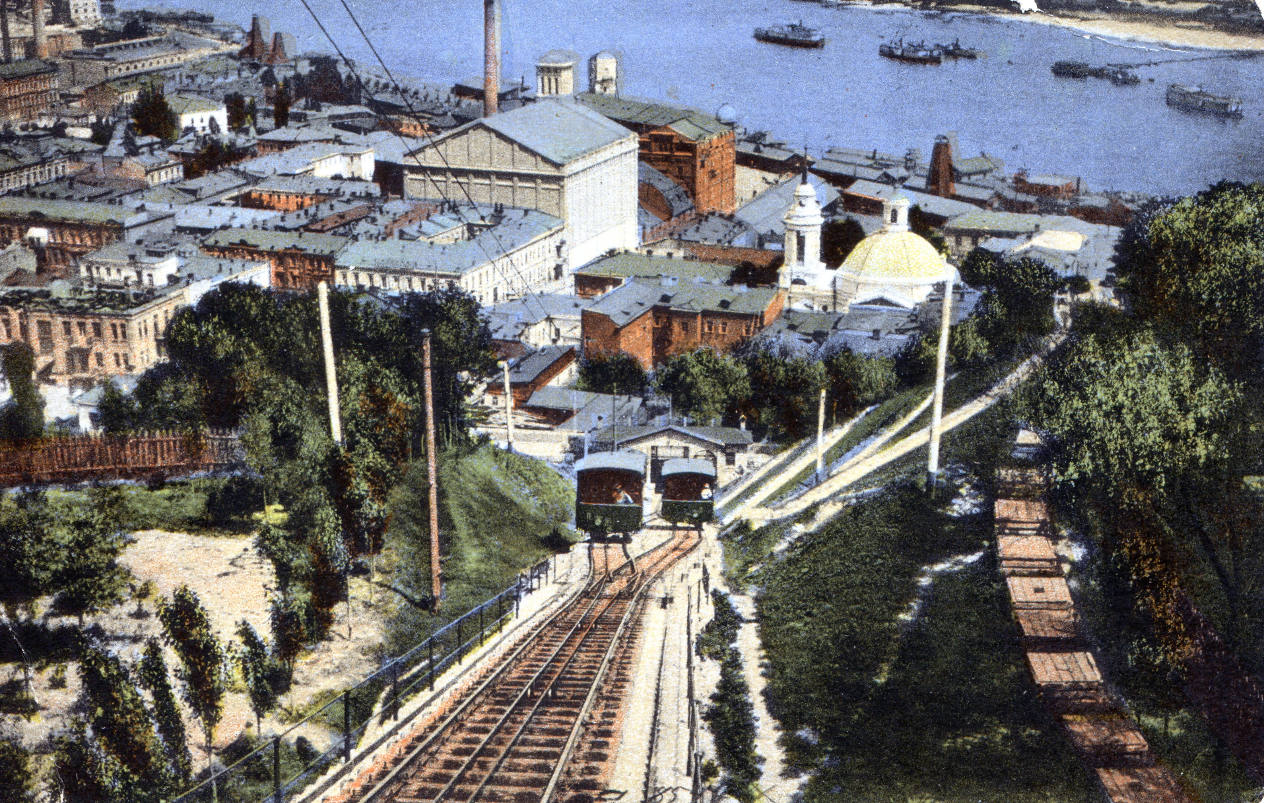
\includegraphics[width=\linewidth]{s-mihpod.jpg}
\end{center}

Старинная открытка с изображением оврага с фуникулером, вид с верхней площадки фуникулера. Собственно, Увоз Боричев.

\vspace*{\fill}

\newpage

\vspace*{\fill}

\begin{center}
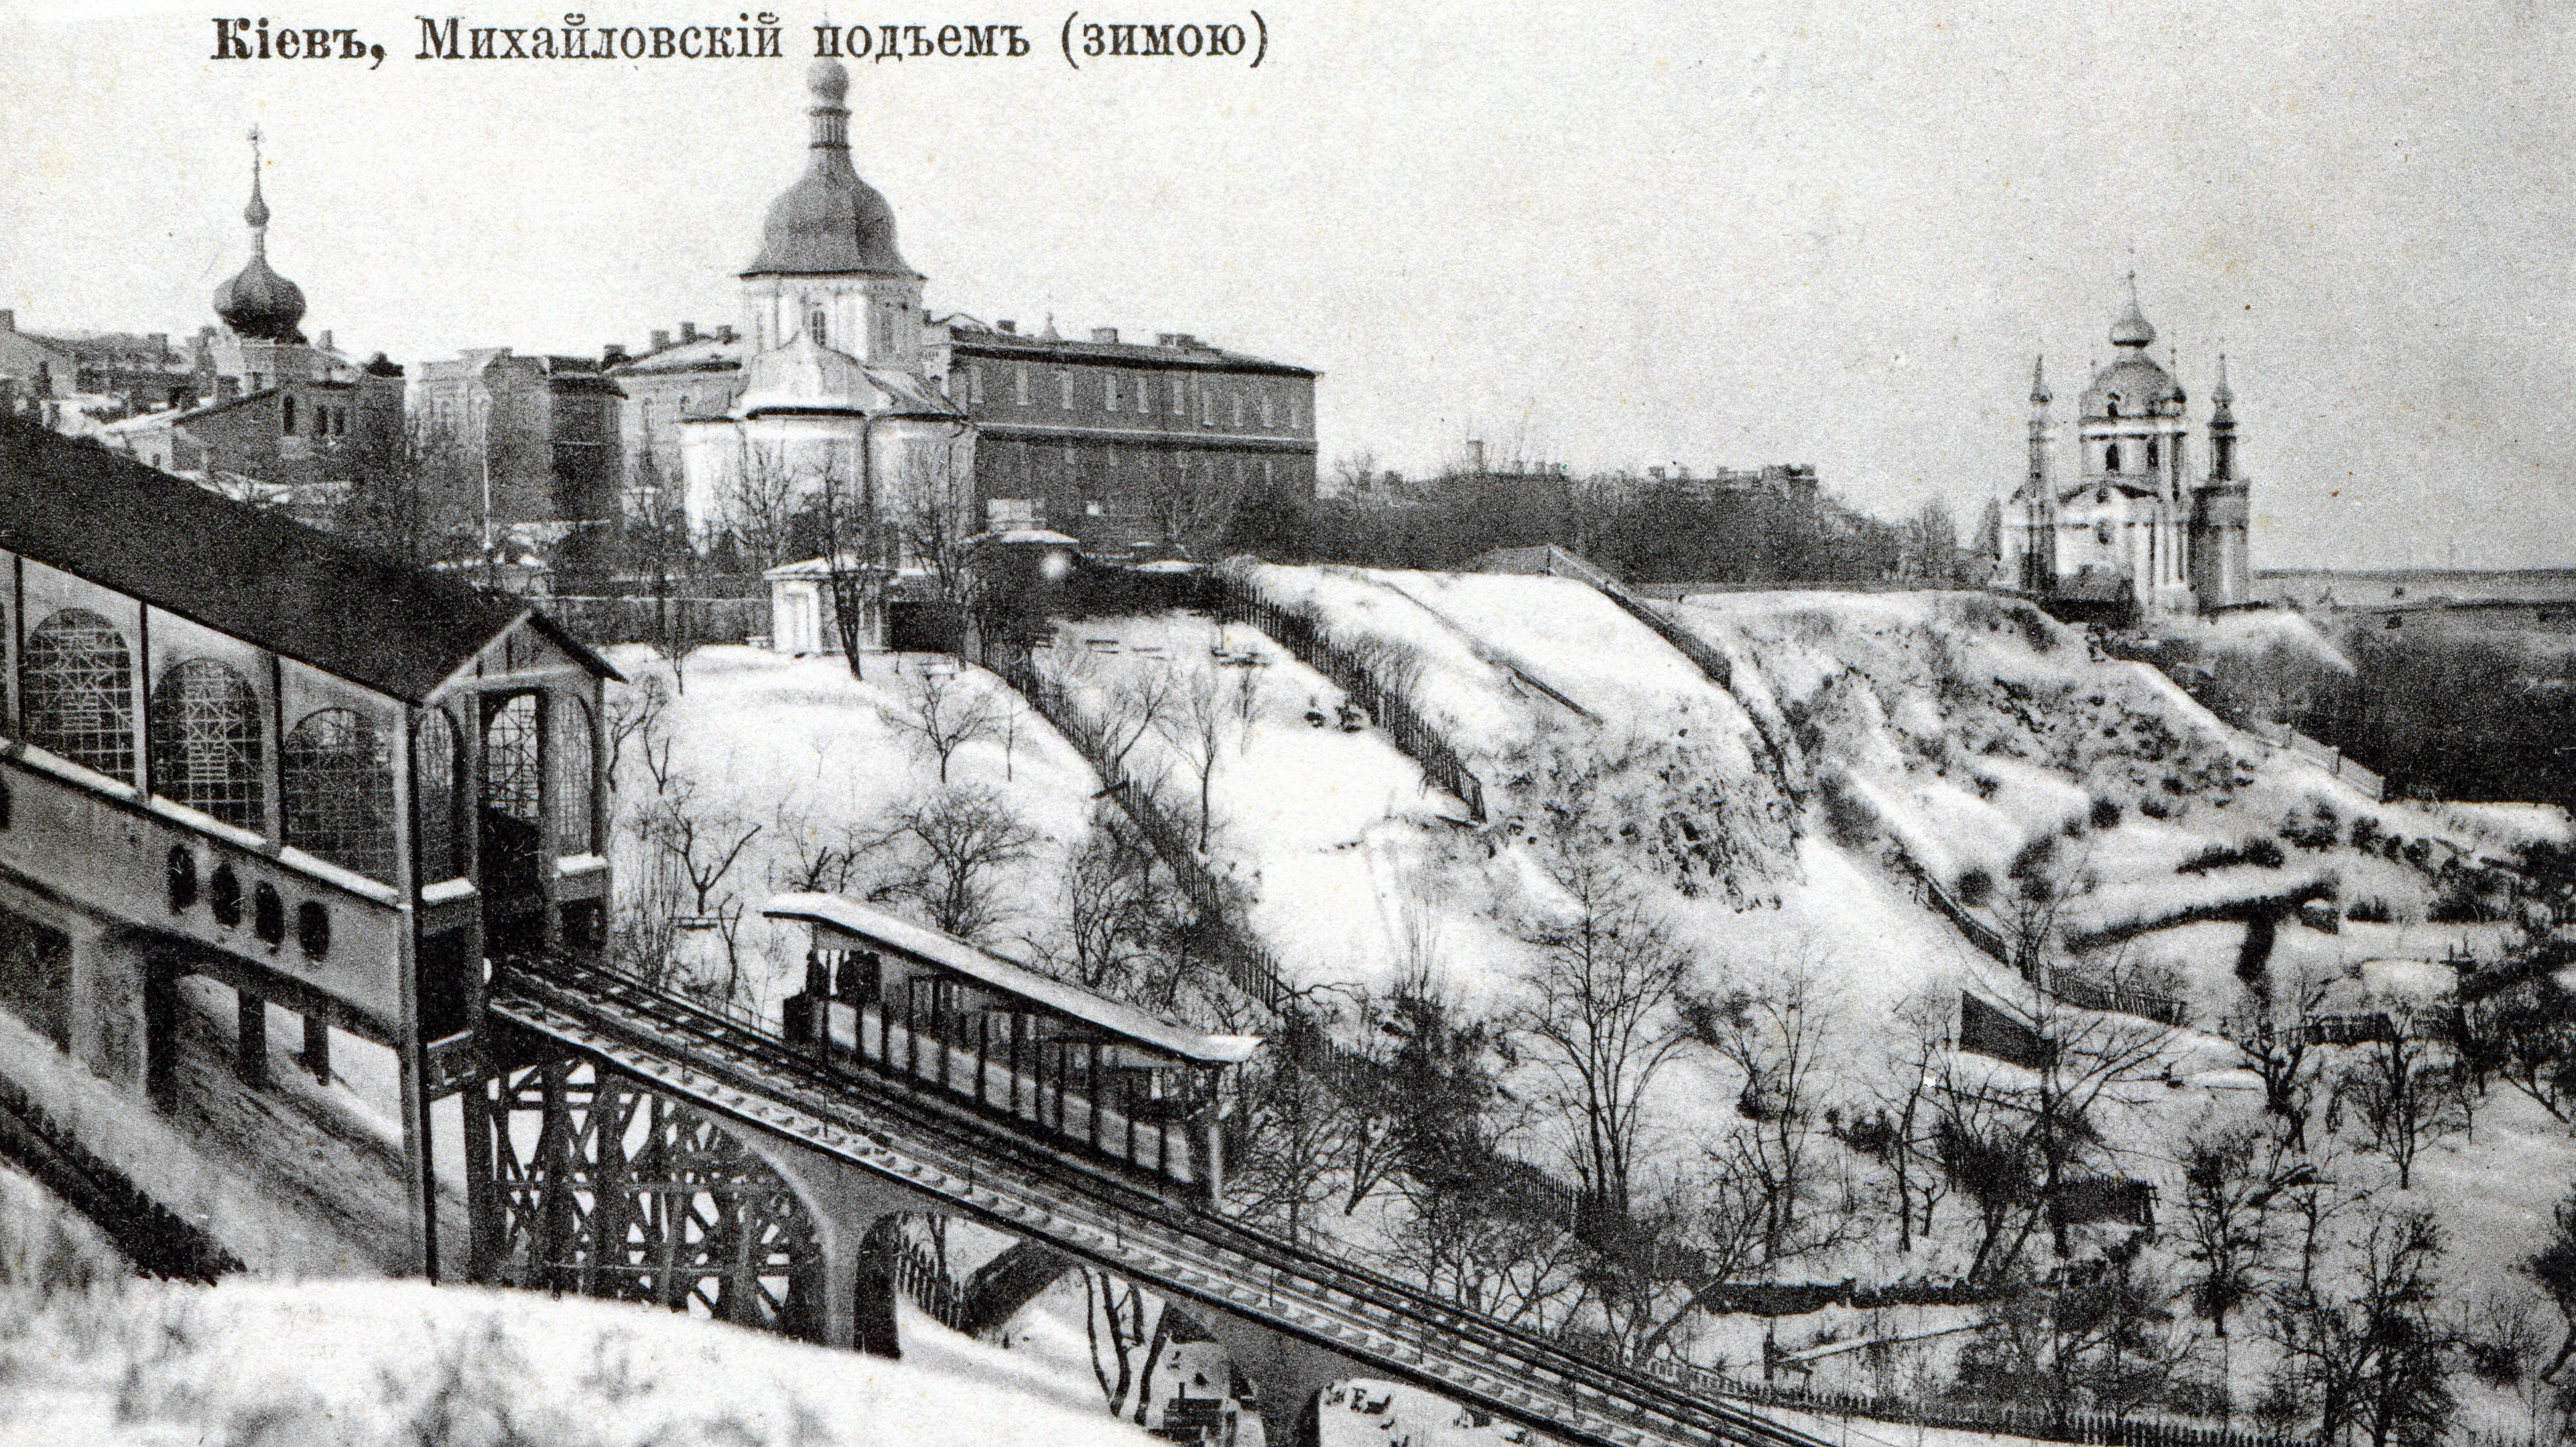
\includegraphics[width=\linewidth]{kuch01.jpg}
\end{center}

Место сада Кучинского на дореволюционной открытке, когда уже само название сада стёрлось из памяти и склоны эти называли Андреевской горой.

На переднем плане – фуникулер, тогда его называли «Михайловский подъем». Овраг над которым едет вагончик и есть Боричев.

За фуникулером – большая Трехсвятительская церковь, возможно на месте давней Васильевской, заложенной Владимиром.

Позади церкви видим здание Женских курсов, а справа в кадре – Андреевская церковь. И вот пространство на уступе между нею и фуникулером, эти склоны, по сути и есть сад Кучинского.

\vspace*{\fill}

\newpage

\vspace*{\fill}

\begin{center}
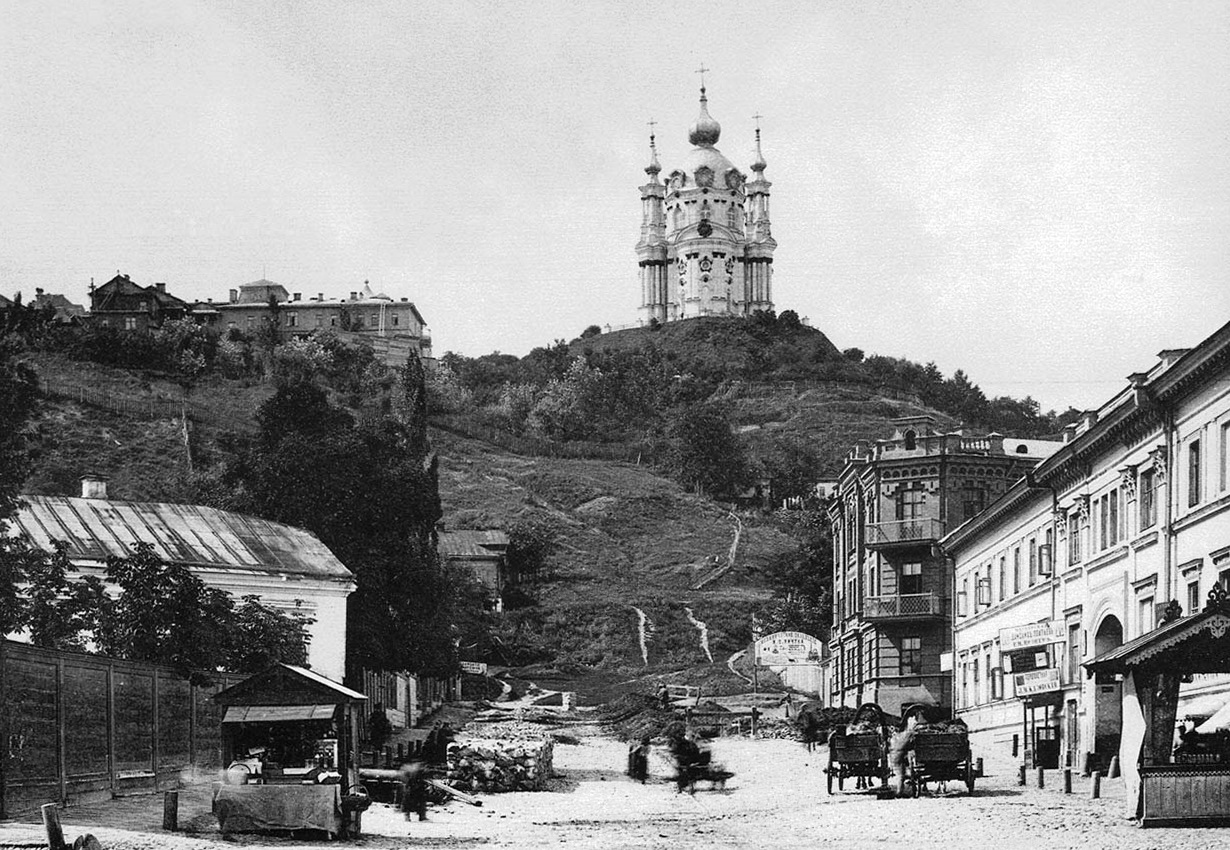
\includegraphics[width=\linewidth]{kuch02.jpg}
\end{center}

Вид с другого ракурса, на Андреевскую церковь, с улицы Андреевской, что на Подоле. Налево видим бывшее место сада Кучинского.

\vspace*{\fill}

\newpage

\vspace*{\fill}


\begin{center}
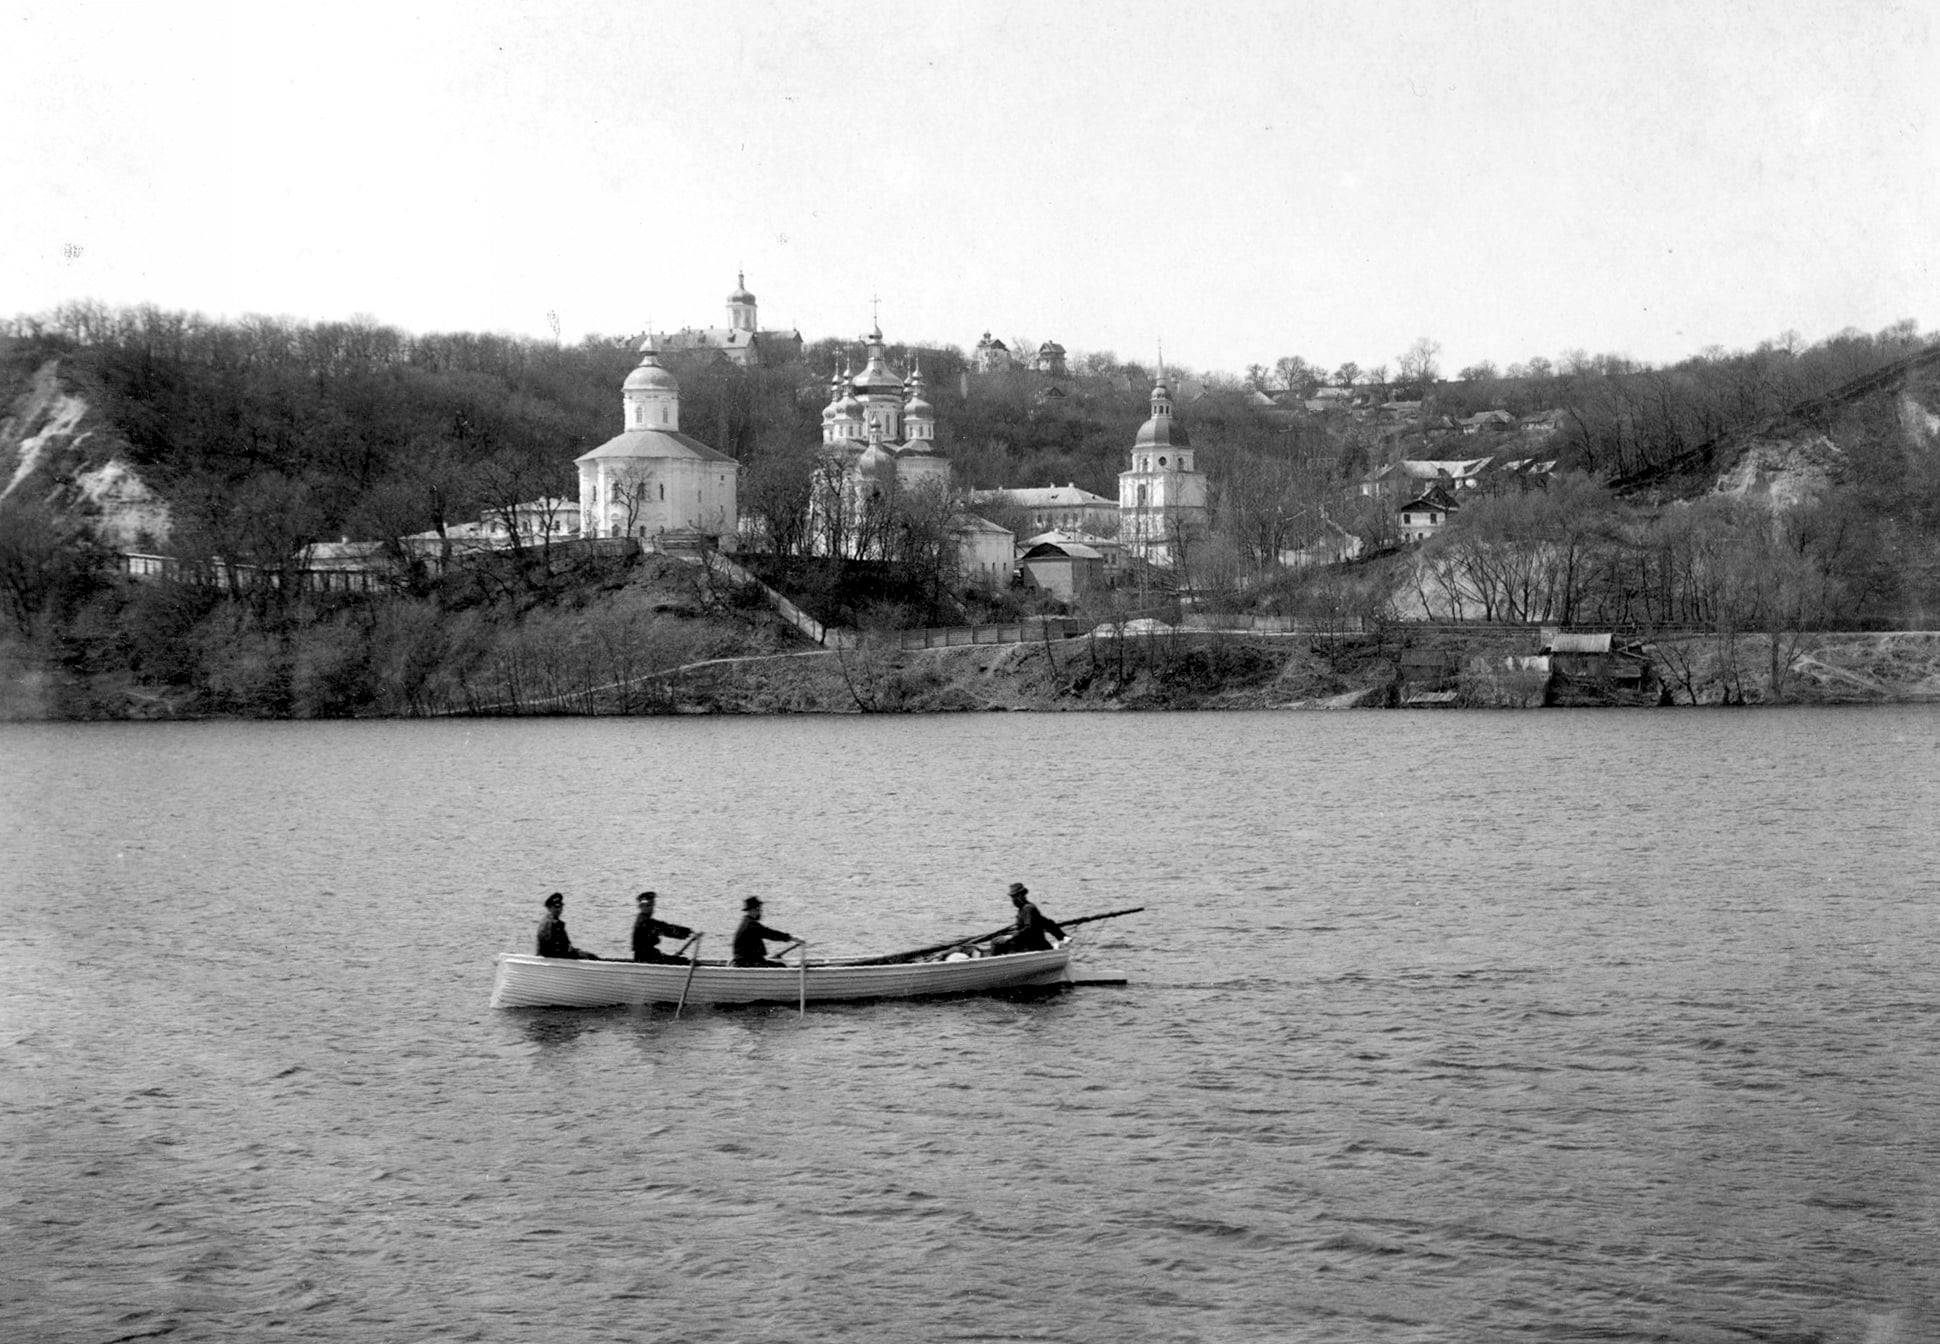
\includegraphics[width=\linewidth]{vyd01.jpg}
\end{center}

Вид на урочище Выдубичи и монастырь. Слева направо – храм чуда св. Михаила в Хонех, Георгиевский собор, Колокольня с церковью пророка Даниила. На горе наверху строения Ионинского Свято-Троицкого монастыря.

\vspace*{\fill}


\newpage

%\backmatter

%\appendix
%\addappheadtotoc


%\input{appendix/dict.tex}

\begin{thebibliography}{999}
\bibitem{zeleninrusalki}
\emph{Избранные труды. Очерки русской мифологии: Умершие неестественною смертью и русалки}. Зеленин Д. К. Индрик, Москва, 1995.

\bibitem{kak}
\emph{Как Владимир идолов низвергал}. Петр Семилетов, DOI 10.5281/zenodo.14212537

\bibitem{volos}
\emph{Скотий бог Волос}. Петр Семилетов, DOI 10.5281/zenodo.14563494
\end{thebibliography}


\end{document} 